\documentclass{article}


%%%%%%%%%%%%%%%%%%%%%%%%%%%%%%%%%%%%%%%%%%%%%%%%%%%%%%%%%%%%%%%%%%%%%%%%%
\pagestyle{plain}                                                      %%
%%%%%%%%%% EXACT 1in MARGINS %%%%%%%                                   %%
\setlength{\textwidth}{6.5in}     %%                                   %%
\setlength{\oddsidemargin}{0in}   %% (It is recommended that you       %%
\setlength{\evensidemargin}{0in}  %%  not change these parameters,     %%
\setlength{\textheight}{8.5in}    %%  at the risk of having your       %%
\setlength{\topmargin}{0in}       %%  proposal dismissed on the basis  %%
\setlength{\headheight}{0in}      %%  of incorrect formatting!!!)      %%
\setlength{\headsep}{0in}         %%                                   %%
\setlength{\footskip}{.5in}       %%                                   %%
%%%%%%%%%%%%%%%%%%%%%%%%%%%%%%%%%%%%                                   %%
\newcommand{\required}[1]{\section*{\hfil #1\hfil}}                    %%
\renewcommand{\refname}{\hfil References Cited\hfil}                   %%
\bibliographystyle{plain}                                              %%
%%%%%%%%%%%%%%%%%%%%%%%%%%%%%%%%%%%%%%%%%%%%%%%%%%%%%%%%%%%%%%%%%%%%%%%%%

\usepackage{graphicx}

\pagestyle{empty}

\begin{document}

\large

\vbox{}
\begin{figure}[!ht]
%\hspace{-4mm}

\includegraphics[width=8cm]{img/logo.png}
\vspace{18mm}
\end{figure}

\begin{figure}[!ht]
\begin{center}
%\hspace{-4mm}
%\hspace{-20mm}
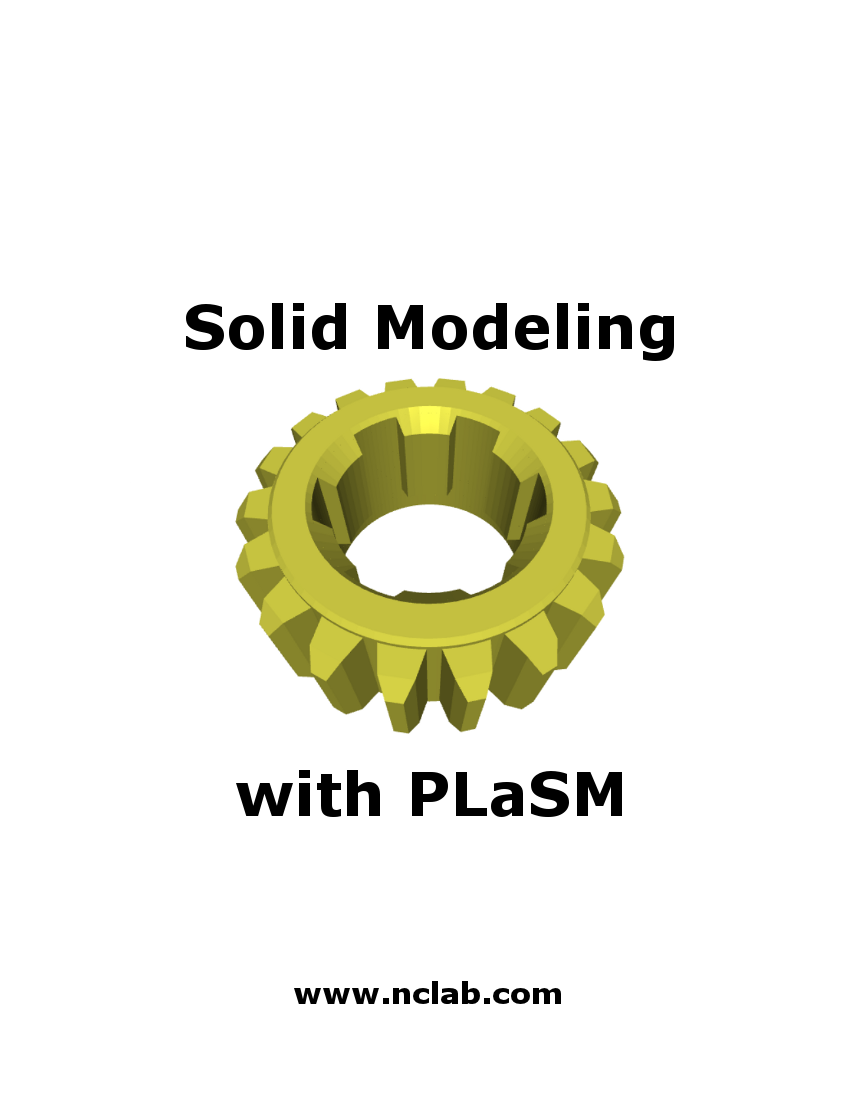
\includegraphics[width=10cm]{img/plasm-frontpage.png}
\vspace{21mm}
\end{center}
\end{figure}

\centerline{\Huge \bf Solution Manual}

\vfill

\centerline{\Large www.nclab.com}

\newpage

%%%%%%%%%%%%%%%%%%%%%%%%%%%%%%%%%%%%%%%%%%%%%%%%%%%%%%%%%%%%%%%%%%%%%%%%%



\section*{}
\small
\input ../common/aboutnclab.tex

%\subsection*{Acknowledgement}
%This publication was created with the help of numerous freely 
%available web resources and tutorials related to Python, Scipy,
%Numpy, Pylab, Matplotlib, Sympy and other projects.

\normalsize

\newpage
%{\ }
\setcounter{tocdepth}{2}
\tableofcontents
%\pagestyle{plain}

\newpage

\pagestyle{plain}
\setcounter{page}{1}


%%%%%%%%%%%%%%%%%%%%%%%%%%%%%%%%%%%%%%%%%%%%%%%%%%%%%%%%%%%%%%%%%%%%%%%%%
\newpage

\pagestyle{plain}

\section{Introduction}

This Solution Manual contains solutions to selected exercises from the 
PLaSM Tutorial. All models presented here are also available for 
cloning via the File Manager's Project $\rightarrow$ Clone menu.

\section{Creating Simple Objects}

\subsection{Blue Brick (A1)}

\begin{verbatim}
# Import PLaSM:
from pyplasm import *

# Define light blue color:
color = [0, 0, 1]

# Create a 3x4x5 brick:
b = CUBOID([3, 4, 5])

# Display the brick:
lab.view(b, color)
\end{verbatim}


\subsection{Red Rectangle (A2)}

\begin{verbatim}
# Import PLaSM:
from pyplasm import *

# Define light red color:
color = [1, 0, 0]

# Create a 3x1 rectangle:
r = CUBOID([3, 1])

# Display the object:
lab.view(r, color)
\end{verbatim}


\subsection{Orange Octahedron (A3)}

\begin{verbatim}
# Import PLaSM:
from pyplasm import *

# Define orange color:
color = [255/255., 140/255., 0/255.]

# Define the points:
points = [[0, -1, 1], [0, 1, 1], [0, -1, -1], [0, 1, -1], \
[2, 0, 0], [-2, 0, 0]]

# Create the convex hull:
oct = CONVEXHULL(points)

# Display the object:
lab.view(oct, color)
\end{verbatim}


\subsection{Pink Pentagon (A4)}

\begin{verbatim}
# Import PLaSM:
from pyplasm import *

# Import some things from Numpy:
from numpy import sin, cos, pi

# Define pink color:
color = [1, 0, 1]

# Number of edges on the base circle:
N = 5

# Radius of base circle:
R = 5

# Create the points:
points = []
for i in range(N):
    angle = i * 2. * pi / N
    points.append([R * cos(angle), R * sin(angle)])
    
# Create the convex hull:
penta = CONVEXHULL(points)

# View the object:
lab.view(penta, color)
\end{verbatim}


\subsection{Cyan Cone (A5)}

\begin{verbatim}
# Import PLaSM:
from pyplasm import *

# Import some things from Numpy:
from numpy import sin, cos, pi

# Define cyan color:
color = [0, 1, 1]

# Number of edges on the base circle:
N = 128

# Radius of base circle:
R = 5

# Cone height:
H = 10

# Create the points:
points = []
for i in range(N):
    angle = i * 2. * pi / N
    points.append([R * cos(angle), R * sin(angle), H])

# Add the tip (0, 0, 0):
points.append([0, 0, 0])
    
# Create the convex hull:
cone = CONVEXHULL(points)

# View the object:
lab.view(cone, color)
\end{verbatim}


\subsection{Carmine Cylinder (A6)}

\begin{verbatim}
# Import PLaSM:
from pyplasm import *

# Define carmine color:
color = [150/255., 0/255., 24/255.]

# Number of linear segments on the curved surface:
N = 128

# Radius:
R = 5

# Height:
H = 3

# Create the cylinder
cyl = CYLINDER([R, H])(N)

# View the object:
lab.view(cyl, color)
\end{verbatim}


\subsection{Topaz Tube (A7)}

\begin{verbatim}
# Import PLaSM:
from pyplasm import *

# Define topaz color:
color = [255/255., 200/255., 124/255.]

# Number of linear segments on the curved surface:
N = 128

# Inner radius:
Rin = 1.9

# Outer radius:
Rout = 2

# Height:
H = 4

# Create the tube:
t = TUBE([Rin, Rout, H])(N)

# View the object:
lab.view(t, color)
\end{verbatim}


\subsection{Sand Sphere (A8)}

\begin{verbatim}
# Import PLaSM:
from pyplasm import *

# Define sand color:
color = [238/255., 214/255., 175/255.]

# Number of linear segments on the curved surface:
N = 64

# Radius:
R = 1.0

# Create the sphere:
s = SPHERE(R)([N, N])

# View the object:
lab.view(s, color)
\end{verbatim}


\subsection{Turquoise Torus (A9)}

\begin{verbatim}
# Import PLaSM:
from pyplasm import *

# Define turquoise color:
color = [64/255., 224/255., 208/255.]

# Number of linear segments on the curved surfaces:
N = 64

# Inner radius:
Rin = 3.0

# Outer radius:
Rout = 5.0

# Create the torus:
t = TORUS([Rin, Rout])([N, N])

# View the object:
lab.view(t, color)
\end{verbatim}





\section{Transformations}

\subsection{Kitchen table (B1)}

\begin{verbatim}
# Import PLaSM:
from pyplasm import *

# Some greenish color:
color = [77/255., 107/255., 80/255.]

# Leg width:
lw = 0.05

# Leg height:
lh = 0.80

# Table measures:
ta = 1.20
tb = 1.60

# Table thickness:
tt = 0.02

# Create one leg:
l1 = CUBOID([lw, lw, lh])

# Create other three legs by translation:
l2 = T([1])([ta - lw])(l1)
l3 = T([2])([tb - lw])(l1)
l4 = T([2])([tb - lw])(l2)

# Top:
top = CUBOID([ta, tb, tt])
top = T([3])([lh])(top)

# Put the table together:
table = STRUCT([l1, l2, l3, l4, top])

# Display it:
lab.view(table, color)
\end{verbatim}


\subsection{Tea table (B2)}

\begin{verbatim}
# Import PLaSM:
from pyplasm import *

# Some greenish color:
color = [77/255., 107/255., 80/255.]

# Leg radius:
lr = 0.01

# Leg height:
lh = 0.50

# Table radius:
tr = 0.40

# Table thickness:
tt = 0.01

# Create one leg:
l1 = CYLINDER([lr, lh])(12)

# Create other three legs by translation:
from numpy import sqrt
tr2 = tr/2.
l2 = T([1, 2])([tr2, tr2])(l1)
l3 = T([1, 2])([tr2, -tr2])(l1)
l4 = T([1, 2])([-tr2, tr2])(l1)
l1 = T([1, 2])([-tr2, -tr2])(l1)

# Top:
top = CYLINDER([tr, tt])(64)
top = T([3])([lh])(top)

# Put the table together:
table = STRUCT([l1, l2, l3, l4, top])

# Display it:
lab.view(table, color)
\end{verbatim}

\subsection{Padlock (B3)}

\begin{verbatim}
# Import PLaSM:
from pyplasm import *

# Some greenish color:
color = [0.9, 0.9, 0.9]

# Base ellipse:
ra = 3
rb = 1

# Base height:
h = 4

# Torus radii:
rin = 2
rout = 2.5
 
# Create base.
base = CYLINDER([ra, h])(64)
base = S(1)(rb/float(ra))(base)
 
# Torus:
t = TORUS([rin, rout])([64, 32])
t = R([1, 3])(PI/2)(t)
t = T([3])([h])(t)

# Padlock:
p = STRUCT([base, t])
  
# Display it:
lab.view(p, color)
\end{verbatim}

\subsection{Bottle (B4)}

\begin{verbatim}
# Import PLaSM:
from pyplasm import *

# Some greenish color:
color = [0, 0.6, 0]

# Base radius:
r = 4.0

# Base height:
h = 20.0

# Neck radius and height:
rn = 1.25
hn = 8.0

# Create base.
base = CYLINDER([r, h])(64)

# Create spherical part:
s = SPHERE(r)([32, 32])
s = T([3])([h])(s)
 
# Create neck:
n = CYLINDER([rn, h + r + hn])(32)
  
# Padlock:
b = STRUCT([base, s, n])

# Rotate 90 degrees:
b = R([1, 3])(-PI/2)(b)
  
# Display it:
lab.view(b, color)
\end{verbatim}


\section{Binary Operations}

\subsection{NCLab icon (C1)}

\begin{verbatim}
# Import PLaSM
from pyplasm import *

color = [0.9, 0.9, 0.9]

c = CUBE(4)
c = DIFF([T([1, 2])([-1, -1])(c), c])
d = T([1])([-1])(CUBOID([4, 2, 3]))
c = DIFF([c, d])
e = T([2, 3])([-1, 1])(CUBOID([4, 4, 2]))
c = DIFF([c, e])

lab.view(c, color)
\end{verbatim}



\subsection{Drilled Cube (C2)}

\begin{verbatim}
from pyplasm import *
size = 2.0
radius = 0.8
color = [0.9, 0.9, 0.9]
subdiv = 64
c = CUBE(size)
c = T([1, 2, 3])([-size/2., -size/2., -size/2.])(c)

height = size + 2.
cyl = CYLINDER([radius, height])(subdiv)
cyl = T([3])([-height/2.])(cyl)

c2 = DIFF([c, cyl])

cyl2 = R([1, 3])(PI/2)(cyl)

c3 = DIFF([c2, cyl2])

cyl3 = R([2, 3])(PI/2)(cyl)

c4 = DIFF([c3, cyl3])
\end{verbatim}


\subsection{Ashtray (C3)}

\begin{verbatim}
# Import PLaSM:
from pyplasm import *

# Define color:
color = [0.9, 0.9, 0.9]

# Outer cylinder:
Rout = 10.0
Hout = 3.0
cyl_outer = CYLINDER([Rout, Hout])(128)

# Inner cylinder
Rin = 8.0
Hin = 3.0
bottom_thickness = 0.5
cyl_inner = CYLINDER([Rin, Hin])(128)
cyl_inner = T(3)(bottom_thickness)(cyl_inner)

# Subtract inner cylinder from outer:
out = DIFF([cyl_outer, cyl_inner])

# Tiny cylinder to cut off the radiuses:
Rtiny = 2.0
Htiny = 2 * Rout + 2.0
cyl = CYLINDER([Rtiny, Htiny])(64)

# Lay the first cylinder horizontall over the ashtray:
cyl1 = T([3])([-Htiny/2.])(cyl)
cyl1 = R([1, 3])(PI/2)(cyl1)
cyl1 = T([3])([Rtiny + Hout/2.0])(cyl1)

# Just rotate by 90 degrees about the z axis:
cyl2 = R([1, 2])(PI/2)(cyl1)

# Cutting off the radiuses at once
out = DIFF([out, cyl1, cyl2])
 
# Display the result:
lab.view(out, color)
\end{verbatim}



%\section{Creating Simple Objects (Continued)}
%Coming soon.


%\section{Curves and Curved Surfaces}
%Coming soon.



\section{The Power of Scripting}

\subsection{Aztec Pyramid (D1)}

\begin{verbatim}
# Import PLaSM:
from pyplasm import *

# Color:
color = [0.9, 0.9, 0.9]

# Bottom side length:
BSL = 50.0

# Top side length:
TSL = 20.0

# Height:
H = 20.0

# Number of layers:
N = 10

# Sanity checks:
ok = True
if BSL < TSL: 
    ok = False
if H <= 0:
    ok = False
if N <= 0:
    ok = False

if ok == True:
    h = H / float(N)
    e = BSL
    de = (BSL - TSL) / float(N)
    pyramid = CUBOID([e, e, h])
    for i in range(N-1):
        e -= de
        pyramid = TOP([pyramid, CUBOID([e, e, h])])
    
    lab.view(c, color)
else:
    print "Incorrect input parameters!"
\end{verbatim}

\subsection{Tower of Hanoi (D2)}

\begin{verbatim}
# Import PLaSM:
from pyplasm import *

# Color:
color = [184/255., 115/255., 51/255.]

# Bottom radius:
BR = 40.0

# Top radius:
TR = 10.0

# Height:
H = 60.0

# Number of layers:
N = 8

# Sanity checks:
ok = True
if BR < TR: 
    ok = False
if H <= 0:
    ok = False
if N <= 0:
    ok = False

if ok == True:
    # Thickness: 
    h = H / float(N)

    # Create base plate:
    plate = CUBOID([7 * BR, 3 * BR, h])

    # Create poles:
    p1 = CYLINDER([TR/3., H*1.1])(16)
    p1 = TRANSLATE([1, 2, 3])([1.5 * BR, 1.5 * BR, h])(p1)
    p2 = TRANSLATE([1])([2*BR])(p1)
    p3 = TRANSLATE([1])([2*BR])(p2)
  
    # Create the tower:
    e = BR
    de = (BR - TR) / float(N)
    tower = CYLINDER([e, h])(64)
    for i in range(N-1):
        e -= de
        tower = TOP([tower, CYLINDER([e, h])(64)])
    
    # Put the tower on the plate:
    tower = TRANSLATE([1, 2, 3])([1.5 * BR, 1.5 * BR, h])(tower)
    
    lab.view(STRUCT([plate, p1, p2, p3, tower]), color)
else:
    print "Incorrect input parameters!"
\end{verbatim}


\subsection{Horse Corral (D3)}

\begin{verbatim}
# Import PLaSM:
from pyplasm import *

# This color is called "saddle brown":
color = [139/255., 69/255., 19/255.]

# Pole width:
W = 0.2

# Pole height:
H = 2.0

# Corral radius:
r = 10.0

# Number of sides:
N = 32

# Prototype of a pole:
pole = CUBOID([W, W, H])
pole = T([1, 2])([-W/2., -W/2.])(pole)
pole = T([1])([r])(pole)
 
# Create all poles:
angle = 2 * PI / N
fence = []
for i in range(N):
    fence.append(R([1, 2])(i * angle)(pole))
    
# Prototype of horizontal logs:
from numpy import sin, cos
L = 2 * r * sin(angle / 2)
log = CUBOID([0.05, L, 0.2])
log = R([1, 2])(angle/2)(log)
log = T([1, 3])([r, H/8.])(log)  
log2 = T([3])([H/4.])(log)
log3 = T([3])([H/4.])(log2)

# Append horizontal logs to each pair of 
# adjacent poles:
for i in range(N):
    fence.append(R([1, 2])(i * angle)(log))
    fence.append(R([1, 2])(i * angle)(log2))
    fence.append(R([1, 2])(i * angle)(log3))

# Show the complete fence:
lab.view(STRUCT(fence), color)
\end{verbatim}

\subsection{Wagon Wheel (D4)}

\begin{verbatim}
Coming soon.
\end{verbatim}

\end{document}
